% %%%%%%%%%%%%%%%%%%%%%%%%%%%%%%%%%%%%%%%%%%%%%%%%%%%%%%%%%%%%%%%%% SECTION FIVE
% %%%%%%%%%%%%%%%%%%%%%%%%%%%%%%%%%%%%%%%%%%%%%%%%%%%%%%%%%%%%%%%%%%%%%%%%%%%%%%
\section{Mid-Side}
Harvey Fletcher, fisico americano, autori di numerosi contributi scientifici in
acustica, ingegneria elettrica, linguaggio, musica, fisica atomica, immagini
sonore ed educazione, nel 1934 firma uno degli articoli che compongono il testo
cardine per la storia della tecnologia sonora “\emph{Symposium on Auditory
Perspective}”, sulla percezione e la trasmissione della musica dal vivo del
teatro, che inizia con le seguenti parole:

\begin{quotation}
In this electrical era one is not surprised to hear that orchestral music can be
picked up in one city, transmitted a long distance, and reproduced in another.
Indeed, most people think such things are commonplace. They are heard every
night on the radio. However, anyone who appreciates good music would not admit
that listening even to the best radio gives the emotional thrill experienced in
the concert hall. \cite{hf34}
\end{quotation}

Oggi abbiamo perso ogni scintilla di “quell'era elettrica”, anche quella che ha
suscitato la fiamma di interesse nell'ascolto della musica orchestrale
attraverso la trasmissione

%, o quella che ha suscitato la fiamma di interesse
% nell'ascolto della musica orchestrale, o quella dell'interesse nell'ascolto o,
% molto più semplicemente, la fiamma dell'di interesse. Cento anni dopo quella
% “era” siamo scimmie. Dobbiamo considerare questo fallimento. Inadempienza. Dobbiamo considerare che
% un libro, anche il più inadeguato, in quanto oggetto di pensiero ha potere, come
% dimostrato nell'introduzione, che potrebbe essere il potere di distruggere.

Nel 1964, Paul W. Klipsch introdusse la ristampa del “\emph{Symposium}”:

\begin{quotation}
The following paper is a reprint of one of the most important papers in the
field of audio. Fundamentals do not change. The laws of physics endure. In
reprinting the Symposium, the fundamentals are restated. \cite{sap1964}
\end{quotation}

Il testo di Fletcher \cite{hf34} è datato 1934, un anno dopo l'approvazione
del brevetto Blumlein che descrive il concetto fondamentale di trasmissione e
registrazione del suono Mid-Side. In quell'epoca gli interessi commerciali e
quelli di ascolto erano intrecciati, in una forma \emph{stereo} solida.

Parlando di orecchie e attività cerebrali per determinare la direzione di una
fonte Blumlein ha scritto:

\begin{quotation}
…it is fairly well established that the main factor having effect are phase
differences and intensity differences between the sounds reaching the two ears,
the influence with each of these has depending upon the frequency of the sounds
emitted. For low frequency sound waves there is little or non difference in
intensity at the two ears but there is a marked phase difference. For a give
obliquity of sound the phase difference is approximately proportional to
frequency, representing a fixed time delay between sound arriving at the two
ears, by noting which there is a phase difference of $\pi$ radians or more
between sound arriving at the two ears from a source located on the line joining
them: but above such frequency if phase difference were the sole feature relied
upon for directional location there would be ambiguity in the apparent position
of the source. At the stage however the head begins to became effective as a
baffle and causes noticeable intensity difference between the sounds reaching
the two ears, and it is by noting such intensity difference that brain
determines direction of sounds at higher frequencies\footnote{...è abbastanza accertato che il fattore principale che ha effetto sono le differenze di fase e le differenze di intensità tra i suoni che raggiungono le due orecchie, l'influenza con ognuna di queste ha a seconda della frequenza dei suoni emessi. Per le onde sonore a bassa frequenza c'è poca o nessuna differenza di intensità alle due orecchie ma c'è una marcata differenza di fase. Per dare un'obliquità del suono, la differenza di fase è approssimativamente proporzionale alla frequenza, che rappresenta un ritardo fisso tra il suono che arriva alle due orecchie, notando che c'è una differenza di fase di $ \ pi $ radianti o più tra il suono che arriva alle due orecchie da una sorgente situata sulla linea che le unisce: ma al di sopra di tale frequenza se la differenza di fase fosse l'unica caratteristica su cui si basava per la posizione direzionale, ci sarebbe ambiguità nella posizione apparente della sorgente. Tuttavia, nella fase in cui la testa inizia a diventare efficace come un deflettore e causa una notevole differenza di intensità tra i suoni che raggiungono le due orecchie, ed è notando tale differenza di intensità che il cervello determina la direzione dei suoni a frequenze più alte.} .\cite{ab58}
\end{quotation}

Blumlein, sulla base della conoscenza dei meccanismi sopra esposti, ha formulato
la maggior parte dei principi di base impressi nella storia dello stereo.
L'approccio più basilare allo stereo si basava su semplici differenze di livello
nella riproduzione degli altoparlanti, percepite come differenze di livello e di
fase alle orecchie. Nacque la tecnica della coppia stereo direzionale a
microfono coincidente, la più vicina, senza alcun ritardo tra i canali,
l'ideale per alimentare l'altoparlante con una differenza di ampiezza puramente
tra i canali. Una delle tipiche tecniche stereo pure coincidenti prende il nome
di Blumlein: due figure di gradiente di pressione pura-8. Tuttavia, come esposto
nel brevetto, i soli microfoni disponibili per Blumlein nei suoi primi
esperimenti erano i microfoni non direzionali a pressione. Due microfoni non
direzionali quasi distanziati, anche più vicini, sono in grado di alimentare
segnali identici in ampiezza e diversi in fase. Quindi si concentra su una
strategia per fabbricare la differenza di ampiezza nell'altoparlante dalla
differenza di fase nei microfoni. Il risultato fu la sua matrice di somma e
differenza alla base della tecnica del Mid-Side.

\begin{quotation}
\ldots a system of sound transmission wherein the sound
is receive by two or more microphones, wherein at low frequencies difference in
the phase of sound pressure at the microphone is reproduced as difference in
volume at the loud speaker. [\ldots] two microphones transmitted over individual
channels are adapted to interact [\ldots] consisting in half of the sum and half
of the difference respectively of the original \cite{ab58}
\end{quotation}

La matrice di Blumlein di somma e differenza tra i segnali è bidirezionale.
Quando il canale sinistro e destro di una coppia stereo passa attraverso la
matrice, la somma di entrambi i canali fornisce il segnale Mid tutto in fase,
mentre la differenza produce il segnale laterale sfasato. Tuttavia, quando i
segnali del Mid-Side iniziano a viaggiare attraverso la matrice, la somma di Mid
e Side fornisce la conversione da fase sinistra positiva a ampiezza, mentre la
differenza dà la conversione da fase negativa destra a ampiezza.

Qui le tre righe \emph{Faust} codificano per matrice somma e differenza.%

%--------------------------------------------
%----------------larghezza massima del codice
\begin{lstlisting}
nsum = 0.5*(_+_);
ndif = 0.5*(_-_);
sdmx = _,_ <: nsum, ndif;
\end{lstlisting}

%%%%%%%%%%%%%%%%%%%%%%%%%%%%%%%%%%%%%%%%%%%%%%%%%%%%%%%%%%%%%%%%%%%% SECTION SIX
%%%%%%%%%%%%%%%%%%%%%%%%%%%%%%%%%%%%%%%%%%%%%%%%%%%%%%%%%%%%%%%%%%%%%%%%%%%%%%%%
\section{Mid-Side Panner}
\label{sec:mspanner}

L'oggetto \emph{panner} è rappresentato da un potenziometro di controllo
(hardware o software, in entrambi i casi a controllo analogico o digitale). Tale
controllo regola la distribuzione di un segnale sonoro in un campo sonoro stereo o multicanale. Ogni tipica console di registrazione ha un \emph{panpot} per
ciascun canale sorgente in ingresso (abbreviazione di “potenziometro di
panoramica”).

Ogni panner ha un'architettura interna che determina la quantità e la condizione
del segnale sorgente per ogni bus di destinazione. I più semplici suddividono i
segnali audio in canali sinistro e destro, ciascuno dotato di un proprio
controllo di guadagno (volume) discreto. La distribuzione dell'energia tra i due
canali è chiamata legge ed è descrivibile con una funzione matematica.

Come descritto da Blumlein, la sola variazione di ampiezza nella rappresentazione
del panorama stereofonico è solo una parte della complessa percezione binaurale.
Per questo motivo, prima di arrivare a quelli che sono i modelli universalmente
implementati su tutti i mixer del pianeta, è più opportuno riprendere da dove
egli stesso è partito. Ci sono diverse motivazioni per non seguire le mode, la
più affascinante è quella di scoprire che ci sono delle alternative che si possono
rivelari inevitabilmente migliori. La visione di Blumlein fu quella ripresa in
seguito da Gerzon per descrivere il mondo ambisonic, che resta un modo di
descrivere il mondo sonoro percepito e riprodotto in un modo completamente diverso.

L'ultima precisazione riguarda il movimento panoramico. La distribuzione dell'energia
o la condizione della coppia di segnali che regola il movimento panoramico troppo
spesso sono descritti come la possibilità di muovere gli oggetti attorno alla posizione
dell'ascoltatore. Generalmente il panner viene descritto come un pomello che
permette di muovere i suoni da destra a sinistra nel panorama. Se ci fermiamo però ad analizzare il problema, il movimento del suono prodotto da un oggetto acustico tra destra e sinistra di un eventuale panorama, emergono subito diversi problemi. Il primo riguarda l'effetto doppler: se un mezzo con la sirena accesa percorre la strada davanti al mio viso ne percepisco la variazione in frequenza, tipica, dovuta all'effetto doppler: il suono aumenta la frequenza mentre si avvicina a me e poi la diminuisce allpontanandosi. Se applico un movimento di panning ad un suono di sirena fisso, posso muovermi veloce quanto voglio con il pomello, non ne ottengo variazioni in frequenza. Un altro problema del pensare il panning come un movimento della sorgente è relativo al suo environment. Che movimento è un movimento che non tiene conto del luogo in cui il suono si trova? Se un avvocato pronuncia la sua arringa in tribunale parlando ad alta voce e camminando a destra e a sinistra, è inevitabile che se ne percepisca la varaizione topologica, morfologica. A sinistra ho le finestre, a destra un muro in cemento, ecc.
Quindi, arrivando al punto, il panpot nella sua descrizone della condizione dei canali che ricevono i suoi suegnali, non muove la sorgente nello spazio, ma regola la posizione della testa in relaizone ad una sorgente fissa. Un panner, muove langolo di incidenza del suono, ruota la testa, nei confronti della sorgente fissa. 

Prima di inoltrarsi nella stesura di quello che può essere il progetto di un
panner basato sulle equazioni che descrivono la stereofonia MID-SIDE, è
necessario comprendere il significato dela forma polare di un segnale.

Il diagramma polare (o curva polare) è invece un grafico a disegno circolare
dove i parametri sono dati dall’ampiezza e dall’angolo d’incidenza, mentre le
frequenze sono rappresentate da famiglie di curve. In presenza di un’unica curva,
si intende che questa è riferita ad una frequenza di $1KHz$. %piero

Un singolo segnale, nella sua oscillazione, espressa nella variazione di ampiezza
attorno allo zero, potrebbe essere derivato da qualsiasi tipo di microfono senza
un significato particolare. Potrebbe essere generato elettricamente da un
microfono con modello polare particolare o da una fonte sintetica senza
alcuna rilevanza specifica. La provenienza polare, la forma che assume la fase
del segnale, diventa rilevante nel confronto tra segnali.

Il diagramma polare di un microfono che, per caratteristiche costruttive, non
percepisce variazioni di angolo di incidenza del segnale, quindi non-direzionale,
è definito comunemente come omnidirezionale, la sua equazione contiene solo
variazioni di ampiezza, derivate della variazione di pressione dell'aria

\begin{equation}
ndp = 1(x)
\label{eq:omni}
\end{equation}

\begin{figure}[h]
\centering
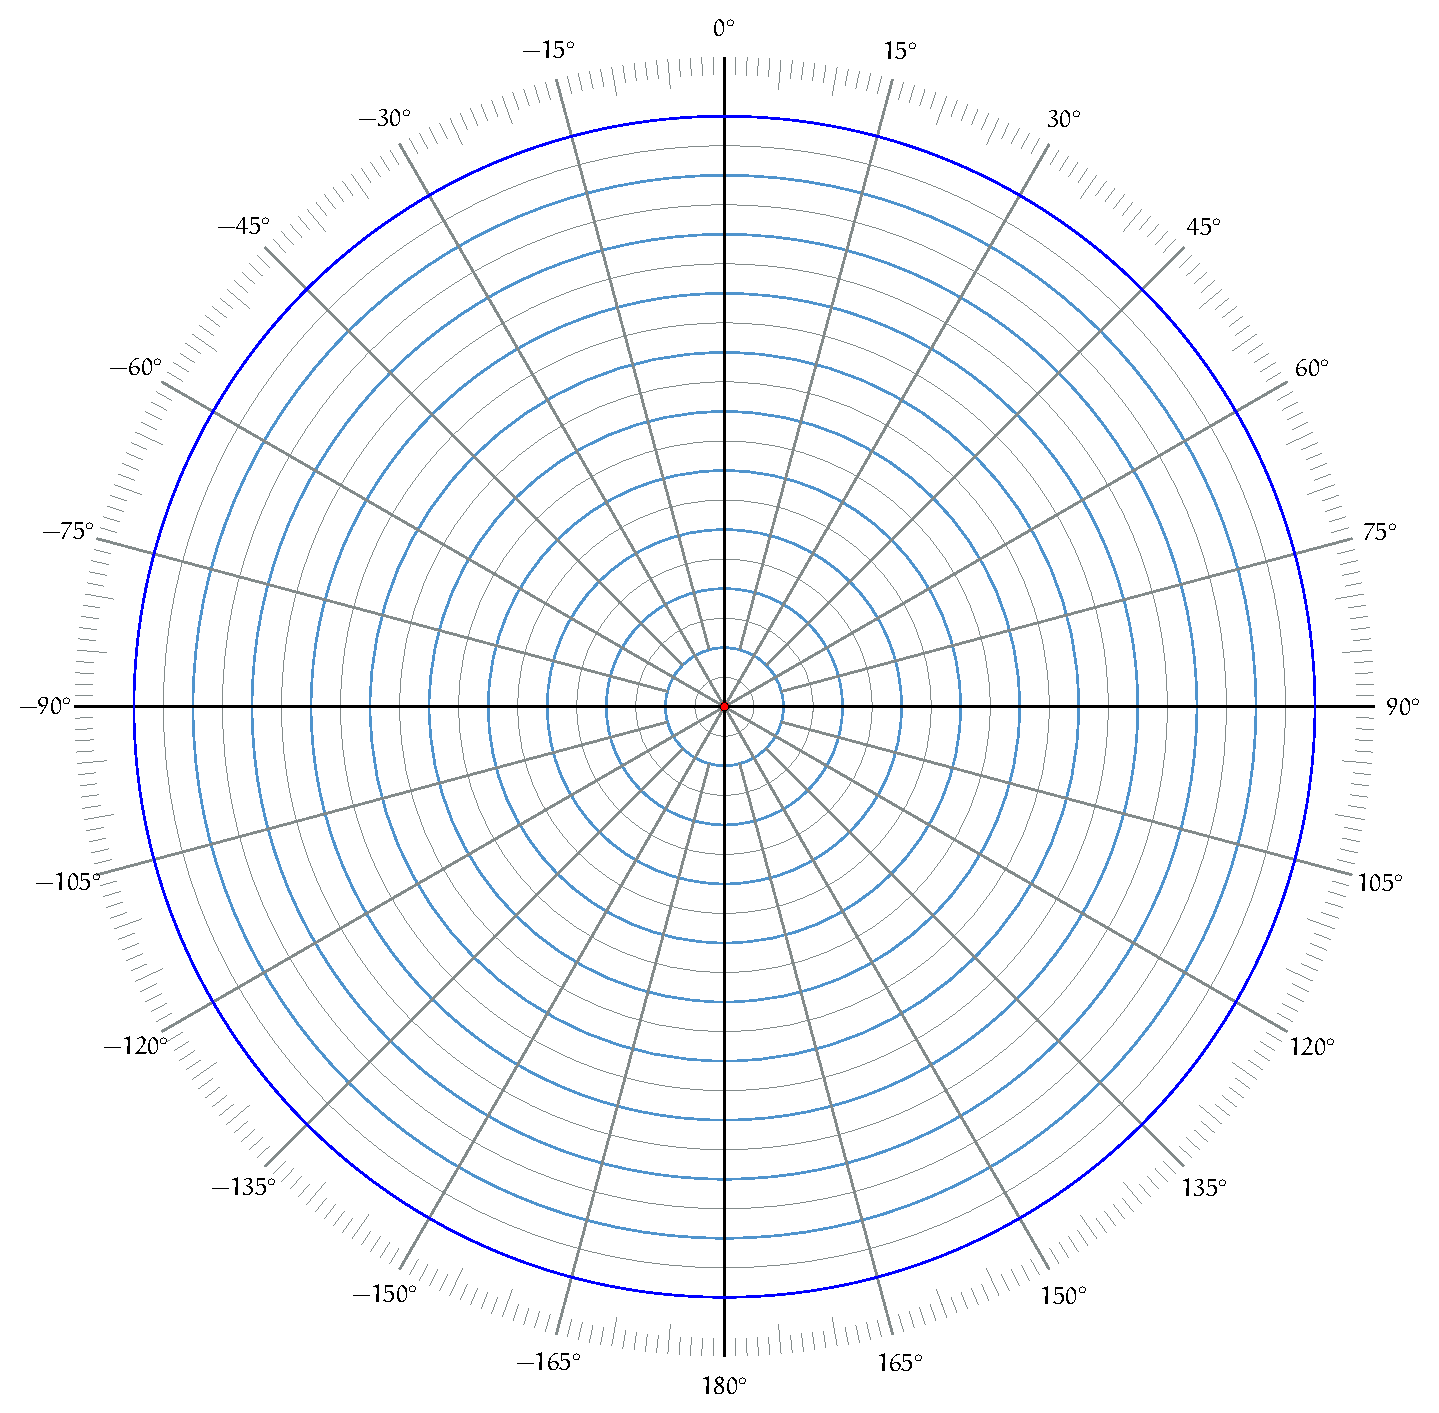
\includegraphics[width=1\columnwidth]{CAPITOLI/_TIKZ/POLAR/omni}
\caption{non-directional}
\label{polar:omni}
\end{figure}

%Il disegno nella parte sinistra di fig. 8 rappresenta la struttura di un tipico microfono a pressione (pressure microphone) omnidirezionale, mentre nella parte destra è rappresentata la sua curva polare, dove vediamo che la direzionalità del suono inizia ad essere percepita dal microfono a partire da circa 5 KHz in su, mentre le frequenze gravi non sono indicate in quanto assimilabili a quella rilevata a 1 KHz, cioè con attenuazione zero per qualsiasi angolo di provenienza del suono.

Dalla descrizione di Blumlein di \emph{Mid-Side}, abbiamo un canale frontale
\emph{Mid} comunemente descritto da un microfono cardioide. Il microfono
cardioide del primo ordine potrebbe essere descritto come una somma delle
variazioni di pressione non direzionale (\emph{ndp})

and bidirectional pressure gradient variations.

\begin{equation}
bpg = x\cos\theta
\label{eq:fig8}
\end{equation}

\begin{figure}[h]
\centering
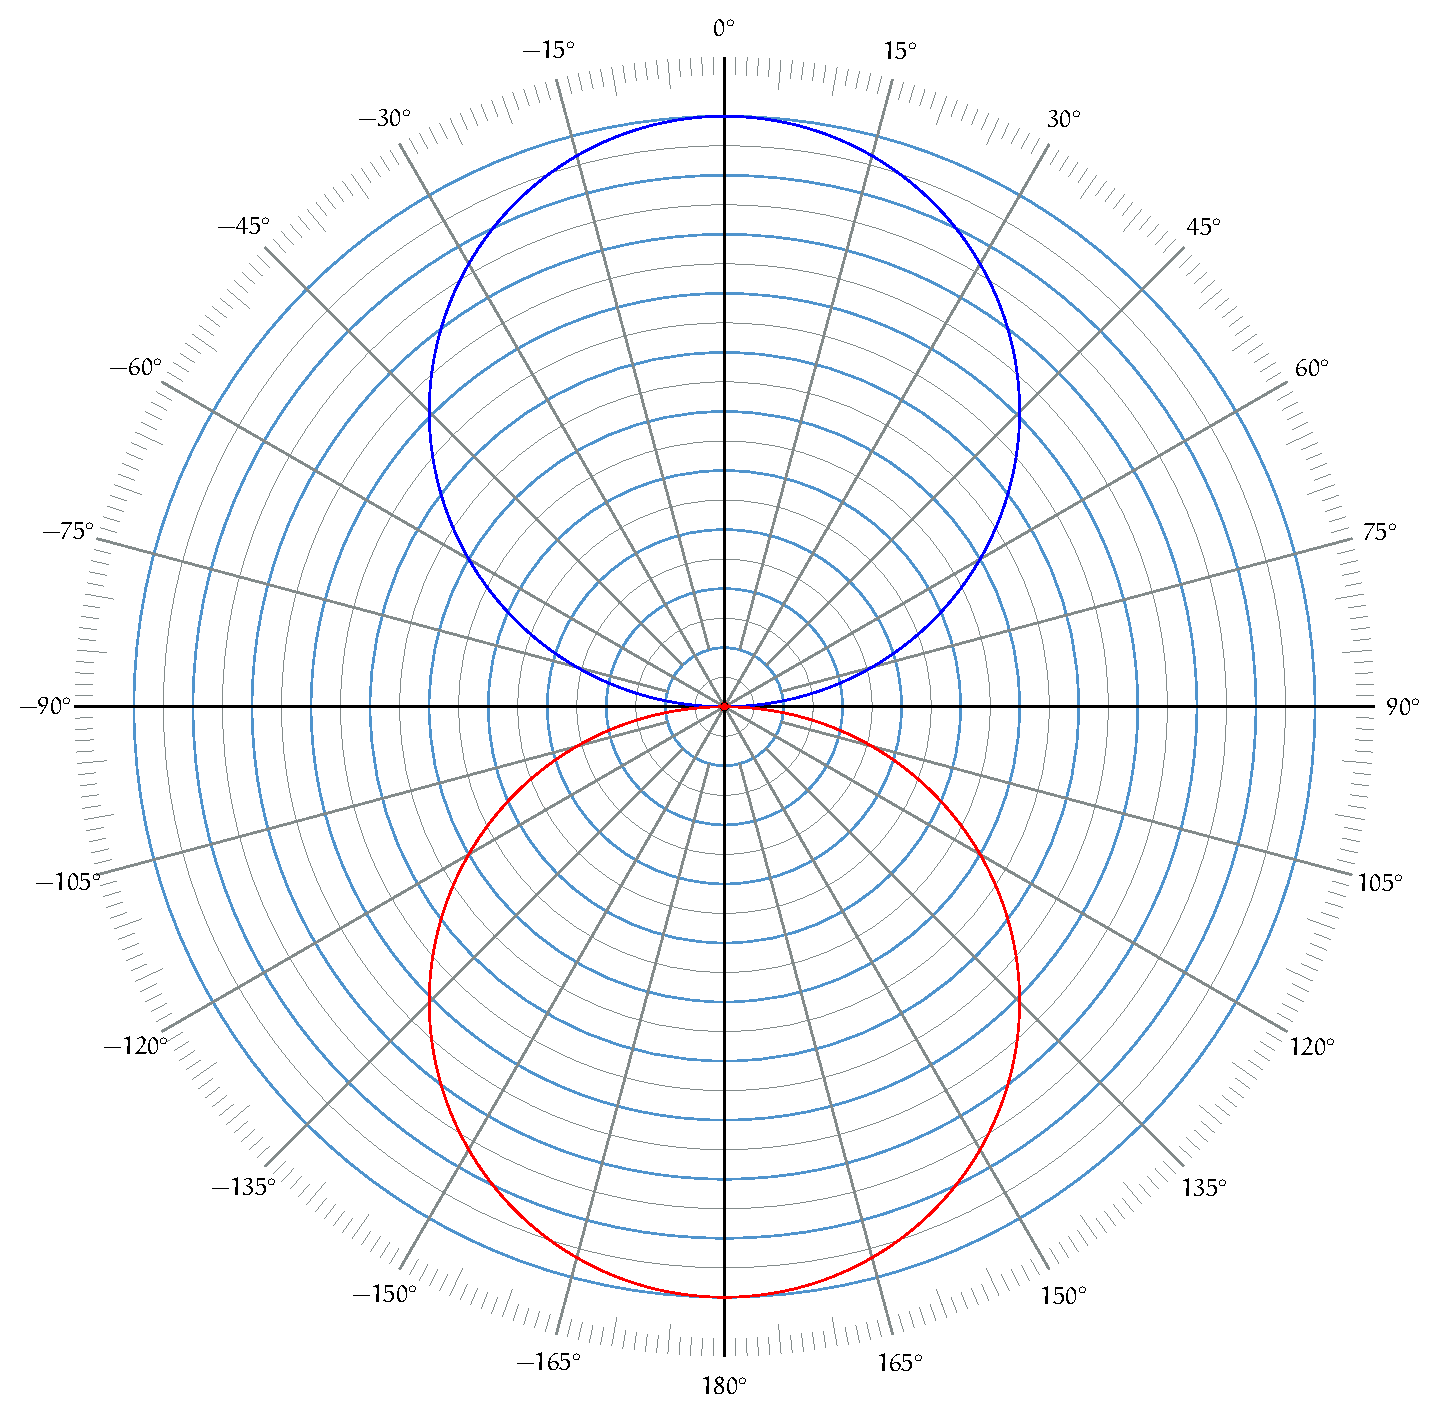
\includegraphics[width=1\columnwidth]{CAPITOLI/_TIKZ/POLAR/fig8}
\caption{Figure-8}
\label{polar:fig8}
\end{figure}

La prima differenza rilevante tra un'equazione del modello polare non
direzionale (\ ref {eq: omni}) e una direzionale (\ ref {eq: fig8}) è la
presenza del coefficiente angolare. L'angolo \ emph {theta} nell'equazione
(\ref{eq:fig8}) descrive la direzione di puntamento del microfono bidirezionale
espressa in radianti. $ X $ è il segnale relativo alla pressione.

Il microfono cardioide (\ emph {cpg}) che tentiamo di sintetizzare deve puntare
alla posizione centrale-anteriore che è il riferimento zero radianti.

\begin{equation}
cpg = 0.5(x) + 0.5(x\cos\theta)
\label{eq:cardioid}
\end{equation}

\begin{figure}[h]
\centering
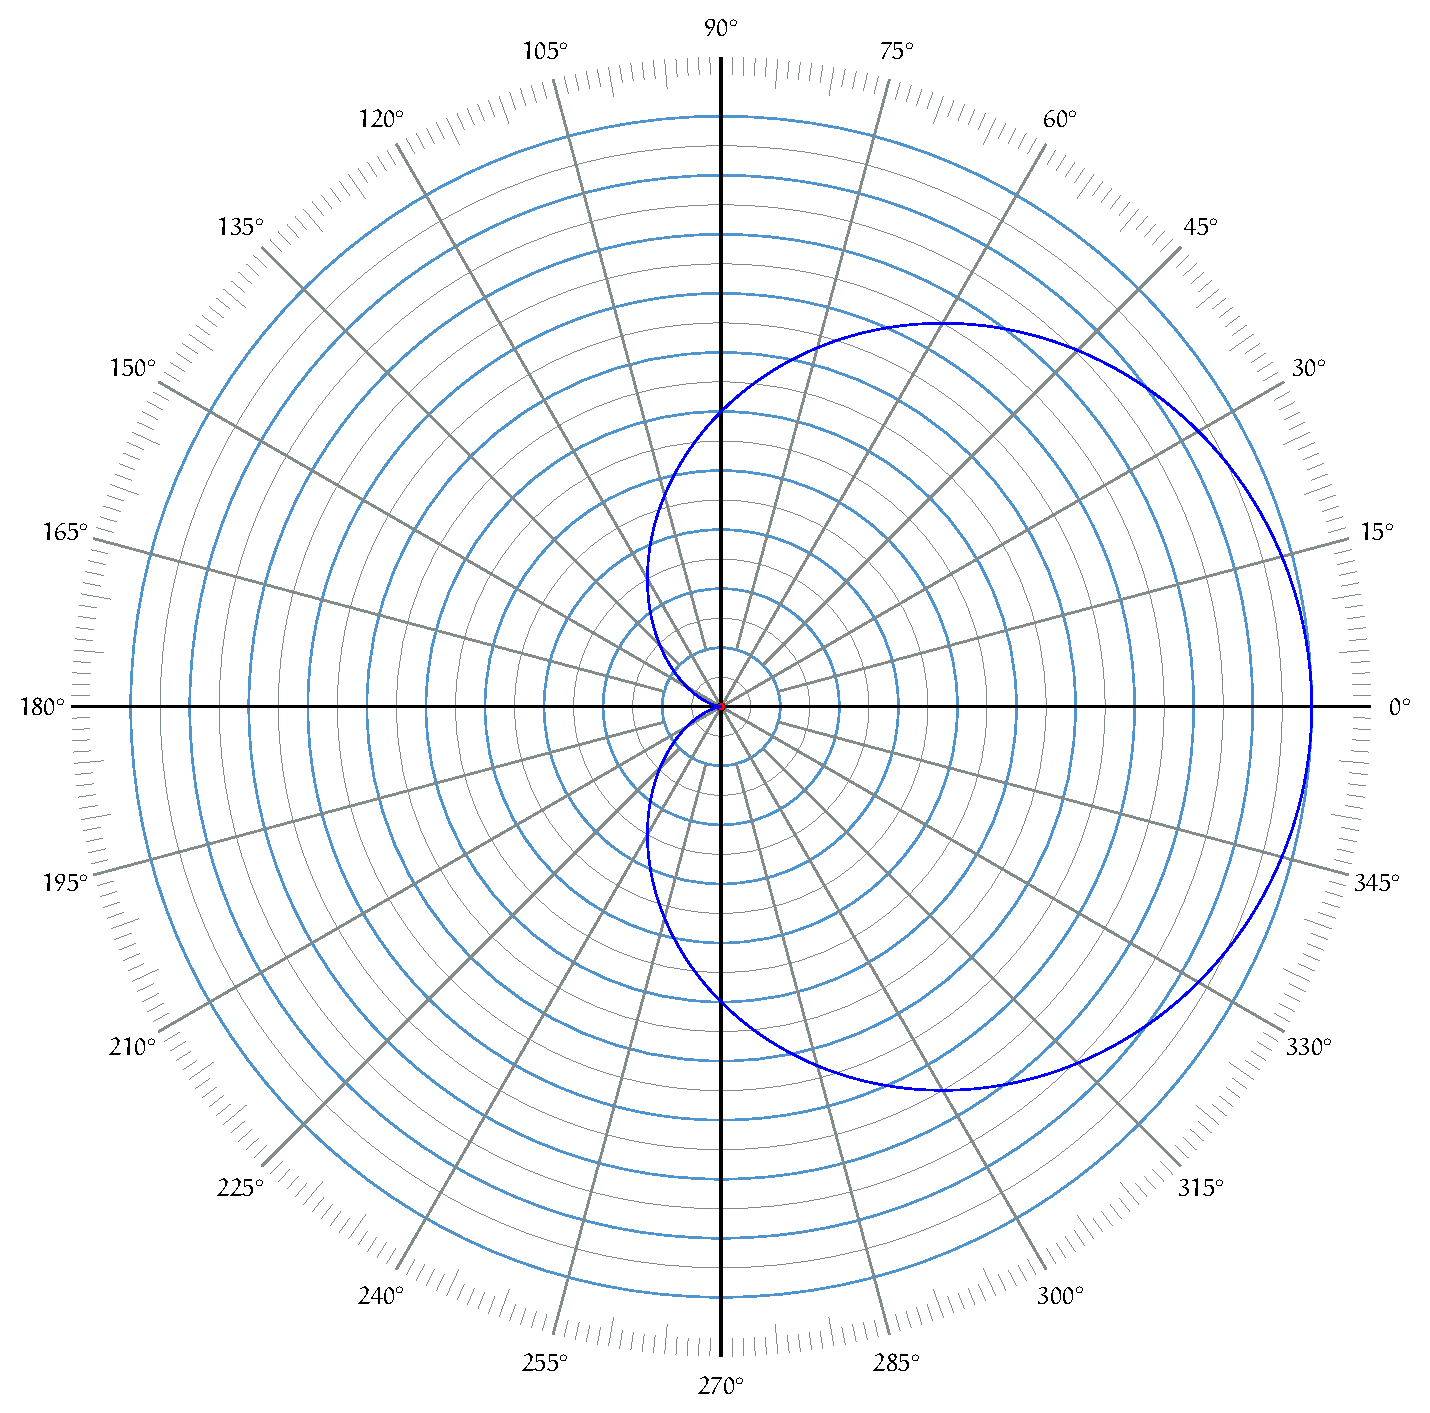
\includegraphics[width=1\columnwidth]{CAPITOLI/_TIKZ/POLAR/cardioid}
\caption{Cardioid}
\label{polar:cardioid}
\end{figure}

Cardioidi e altri schemi più comuni del primo ordine sono prodotti con il
seguente peso tra la pressione non direzionale e il gradiente di pressione
bidirezionale:

\begin{table}[h]
\begin{center}
\begin{tabular}{cc}
Polar Pattern & Equation \\
\hline
Omnidirectional & $ 1(x) $ \\
Subcardioid     & $ 0.75(x) + 0.25(x\cos\theta) $ \\
Cardioid        & $ 0.5(x) + 0.5(x\cos\theta) $ \\
Supercardioid   & $ 0.37(x) + 0.63(x\cos\theta) $ \\
Hypercardioid   & $ 0.25(x) + 0.75(x\cos\theta) $ \\
Bidirectional   & $ 1(x\cos\theta) $ \\
\end{tabular}
\end{center}
\caption{coefficiente \emph{pressione non direzionale} e coefficiente
\emph{gradiente di pressione bidirezionale} per la descrizione dei modelli
polari del primo ordine. Dove $ x $ è il segnale di input, l'angolo di incidenza
della prospettiva $\theta$}
\label{tab:polarcoef}
\end{table}

Quindi dai primitivi schemi polari del primo ordine, non direzionali e
bidirezionali, potremmo derivare, progressivamente, ogni sfumatura di forma tra
di loro, puntando angolarmente ovunque intorno a 2 $ \ pi $ radianti.

Infine, il componente Mid del panner Mid-Side potrebbe essere espresso dalla
formula

\begin{equation}
m(x,p,\theta) = (p*x) + ((1-p)*(x\cos\theta)
\label{eq:mid}
\end{equation}

Dove $ x $ è il segnale di ingresso, $ p $ è il coefficiente di ampiezza, $0.5$
per scopi cardioidi, $\theta$ è la direzione di impatto angolare espressa in
radianti.

Il componente Side è la formula dritta bipolare di figura 8 che punta a sinistra.

\begin{equation}
s(x,\theta) = x*(sin(\theta))
\label{eq:side}
\end{equation}

Il codice Faust per un panner Mid-Side è veramente auto-spiegato: le equazioni
diritte per descrivere sia il cardioide che la figura 8 sono i due componenti
al di fuori del panning.

%--------------------------------------------
%----------------larghezza massima del codice
\begin{lstlisting}
mspan(x,p,rad) = m,s
with{
  m = (p*x)+((1-p)*(x*cos(rad)));
  s = x*(sin(-rad));
};
\end{lstlisting}

\begin{figure}[h]
\centering
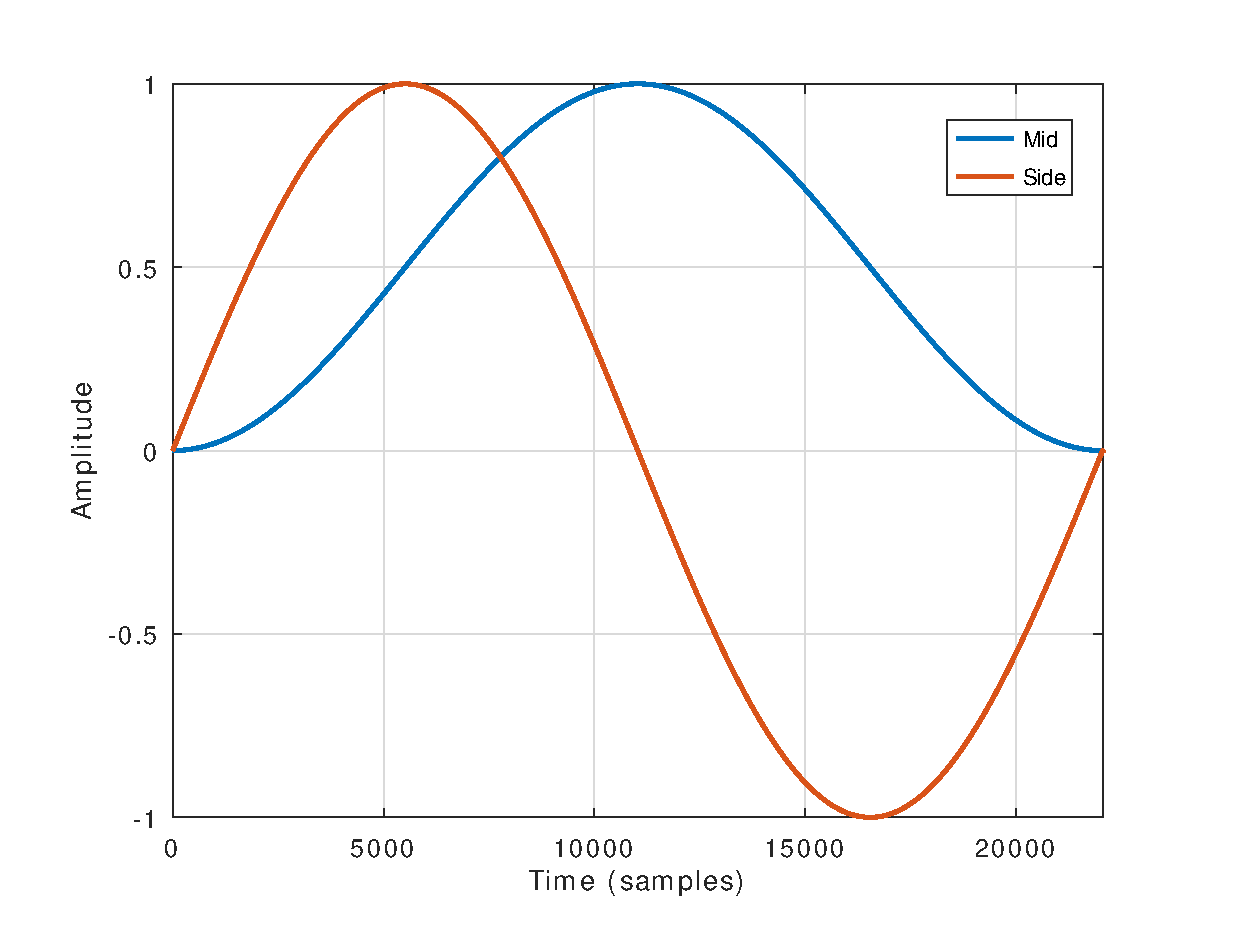
\includegraphics[width=1\columnwidth]{CAPITOLI/1000/IMG/mspan}
\caption{Mid-Side Panner. Il grafico mostra la risposta del panner ad una
variazione di 360 gradi da sinistra (-180 gradi) a destra (180 gradi). La linea
laterale (rossa) mostra la
bipolarità del segnale correlata alle informazioni angolari. La linea Mid (blu)
ha solo energia positiva in relazione alle informazioni angolari. La trama
mostra l'evidenza del significato zero su entrambi i bordi di -180 e 180 gradi,
dove cardioide e figura 8 sono senza ascolto.}
\label{fig:mspan}
\end{figure}

Dobbiamo passare il panner attraverso la matrice della differenza di somma per
ottenere ciò che Blumlein descrive come la differenza di ampiezza nei segnali
degli altoparlanti dalle differenze di fasi.

%--------------------------------------------
%----------------larghezza massima del codice
\begin{lstlisting}
mspan_lr(x,p,rad) = mspan(x,p,rad) : sdmx;
\end{lstlisting}

\subsection{Utilizzi}

Il panner Mid-Side qui proposto non è solo un oggetto tecnico, utile o no,
comparabile o no, relativo ad altri tipi di pan. Il panner Mid-Side qui proposto
è un oggetto di pensiero. Usiamo la tecnica Mid-Side, per riflettere la stessa
stereofonia; perché riteniamo fortemente che alcune circostanze evidenziate
nelle sezioni precedenti debbano essere affrontate, altre migliorate e molte
altre uccise.

Pensare al panning deve essere fortemente incoraggiato perché è un oggetto
semplice troppo spesso usato senza fare domande. La gente può pensare che la
chiave quadratica sia migliore di quella lineare che solo in virtù della sua
introduzione più recente. Ma se interrompiamo il suo “utilizzo senza mettere in
discussione” e, come musicisti, prendiamo il tempo per analizzare l'uso manuale
dell'uno al posto dell'altro, possiamo sentire una differenza, pratica prima del
suono.

Conoscendoli possiamo analizzare il mercato del mixer e il ruolo del pan nella
musica di cultura di massa. Senza un \ -a \ -lys \ -ing questi problemi pratici,
non è davvero comprensibile il motivo per cui la peggiore tecnica di panning sia
mai la maggior parte dell'hardware implementato.

Il codice per costruire un panner di ampiezza quadratica è piuttosto banale.
Il codice più prolisso \ emph {Faust} lo farà in cinque righe. L'eliminazione di
$sqrt$ dalle seguenti formule diventa il panner di ampiezza lineare tradizionale
più semplice.

%--------------------------------------------
%----------------larghezza massima del codice
\begin{lstlisting}
lrpanq(x,p) = l,r
with{
  l = sqrt(1-p)*x;
  r = sqrt(p)*x;
};
\end{lstlisting}

Dove $ p $ è il coefficiente angolare espresso dal potenziometro, in un
intervallo tra $ 0 $ la posizione sinistra, $ 0,5 $ la posizione centrale e $1$
la posizione destra.

Sorridendo, potrebbe essere fatto su una riga:

%--------------------------------------------
%----------------larghezza massima del codice
\begin{lstlisting}
lrpanq(p) = _ <: sqrt(1-p)*_, sqrt(p)*_;
\end{lstlisting}

\begin{figure}[t]
\centering
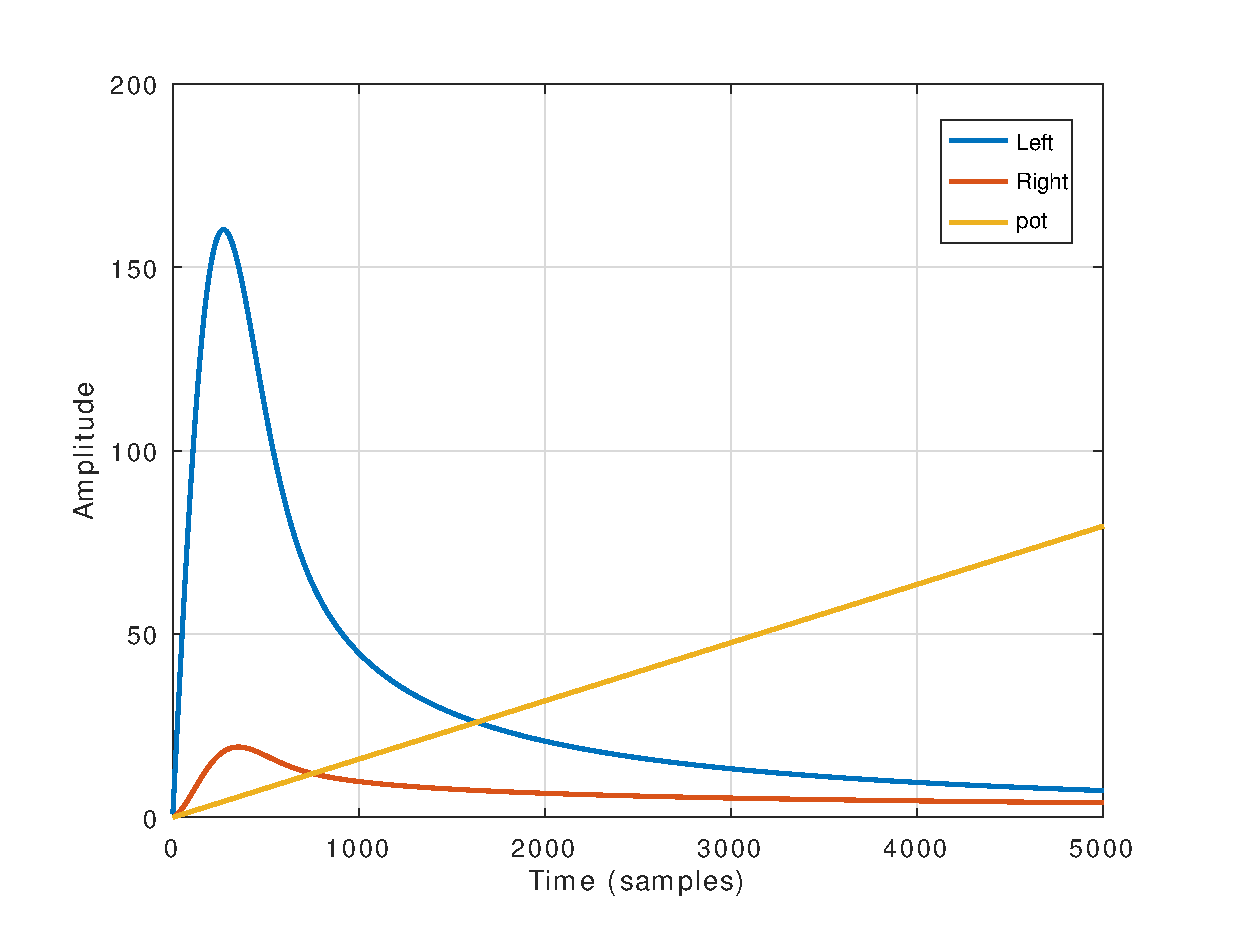
\includegraphics[width=1\columnwidth]{CAPITOLI/1000/IMG/lrpanfb_init}
\caption{\textbf{Risposta feedback panner ampiezza quadratica sinistra-destra}.
La trama mostra la risposta del programmatore in un ciclo di scansione da
sinistra a destra. La trama mostra come l'ampiezza si sposta rapidamente oltre
150 volte il valore iniziale sul canale “in feedback” e oltre 20 volte sul
canale “opposto”.}
\label{fig:lrpanfb1}
\end{figure}

\begin{figure}[t]
\centering
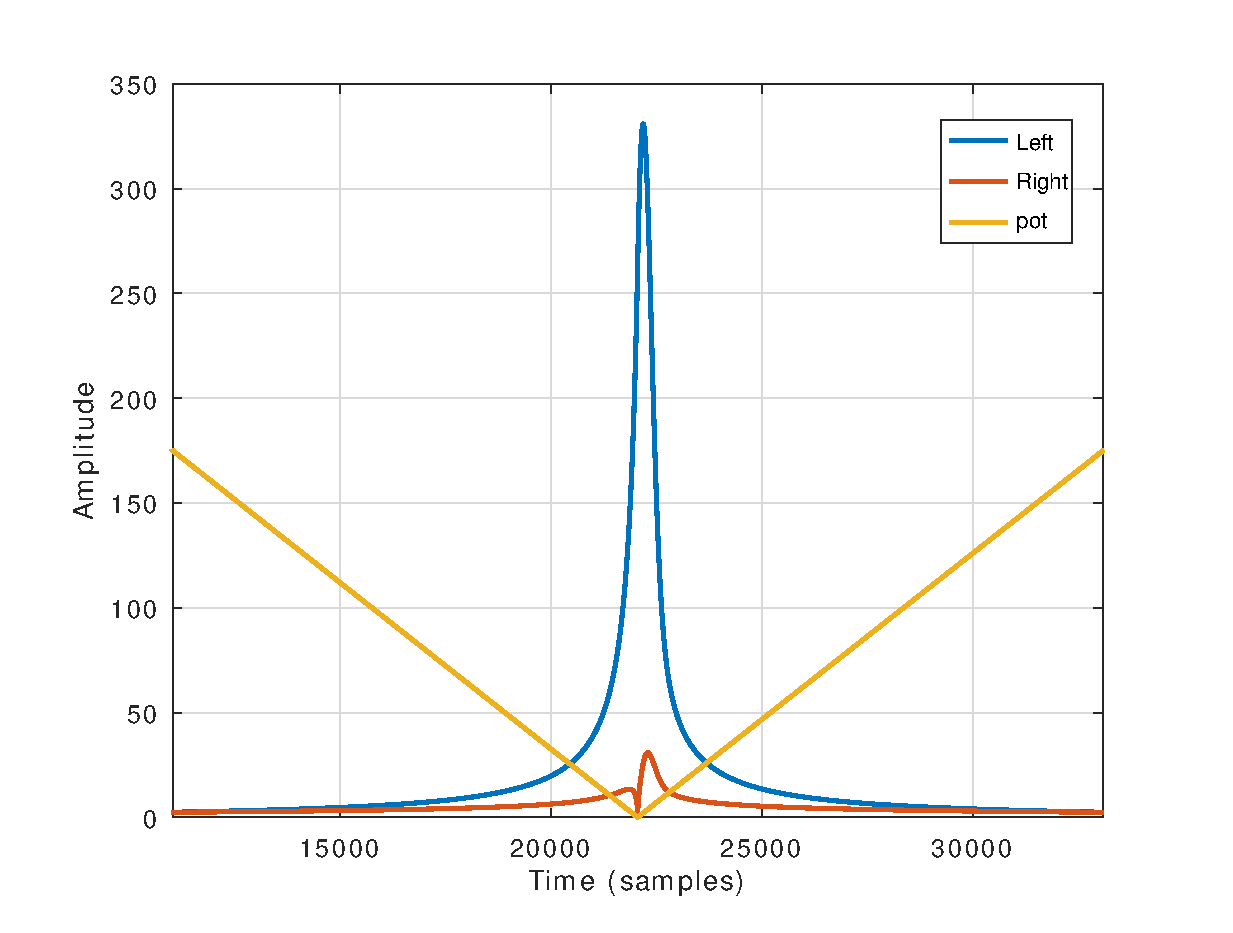
\includegraphics[width=1\columnwidth]{CAPITOLI/1000/IMG/lrpanfbpot2}
\caption{\textbf{Risposta feedback panner ampiezza quadratica sinistra-destra}.
La trama mostra la risposta del programmatore in un ciclo di scansione da
sinistra a destra. La trama mostra come l'ampiezza si sposta rapidamente oltre
150 volte il valore iniziale sul canale “in feedback” e oltre 20 volte sul
canale “opposto”.}
\label{fig:lrpanfb2}
\end{figure}

Abbiamo spiegato il percorso del pan Mid-Side, partendo dalle radici. Ora è il
momento di capire quali sono i possibili utilizzi e quali sono le peculiarità di
un panner Mid-Side invece dei pannolini di ampiezza \emph{tradizionale}.

Il segnale \emph{matrixed} ha la sua complessità come svantaggio. Fermare. In
realtà richiede conoscenza e fantasia per comprendere un segnale come il
significato della combinazione di matrici e richiede anche un po 'di lavoro
complicato più di un segnale diretto.

Come musicisti, anche quando trame e formule appaiono abbastanza chiare, alla
fine, al momento del giudizio, sono le orecchie e l'usabilità musicale a
determinare la scelta migliore, personale.

L'affascinante regno dei segnali \ emph {matrixed} costringe un po 'a lavorare
con il pensiero. Quindi, per noi, ad esempio, la forza di modulazione di fase
del panner Mid-Side aveva suggerito, anche prima di un test pratico, una
migliore stabilità sugli utilizzi dal vivo. Perché? È abbastanza semplice da
dimostrare.

Un microfono viene instradato in un canale, con una chiave appuntita a metà
laterale, supponiamo che 23 gradi a sinistra e inviato agli altoparlanti. Con il
panner quadratico, entrambi i canali sinistro e destro hanno valori di ampiezza
diversi con gli stessi valori di fase. Il feedback dei segnali degli
altoparlanti all'interno del microfono proviene da diverse fonti di energia in
fase. La ricerca del feedback con le dita sul guadagno produrrà segnali che
aumenteranno almeno quadraticamente [fig. \ref{fig:lrpanfb1}, \ref{fig:lrpanfb2}].

\begin{figure}[h]
\centering
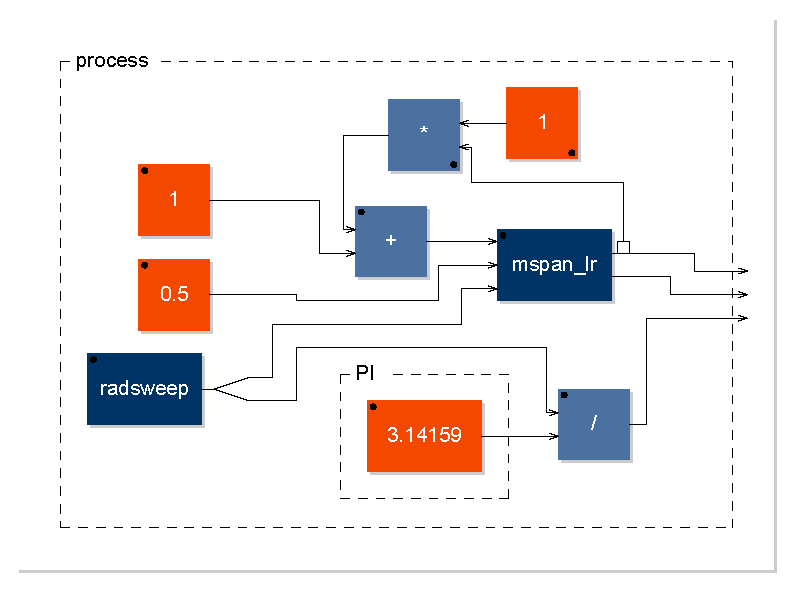
\includegraphics[width=1\columnwidth]{CAPITOLI/1000/IMG/mspanlrfb_diagram}
\caption{\textbf{Block diagram of the infinite feedback}.}
\label{fig:mspanlrfbdiag}
\end{figure}

D'altra parte, nella stessa situazione di feedback, con la stessa provenienza
del panning angolare applicata al segnale del microfono, il pan Mid-Side
produrrà fasi diverse e energia diversa per entrambi gli altoparlanti. Le
differenze, nell'aria, produrranno un modello di feedback più resistivo. In
altre parole, il panner di Mid-Side agisce “naturalmente” come anti-\emph{Larsen}.


\begin{figure}[t]
\centering
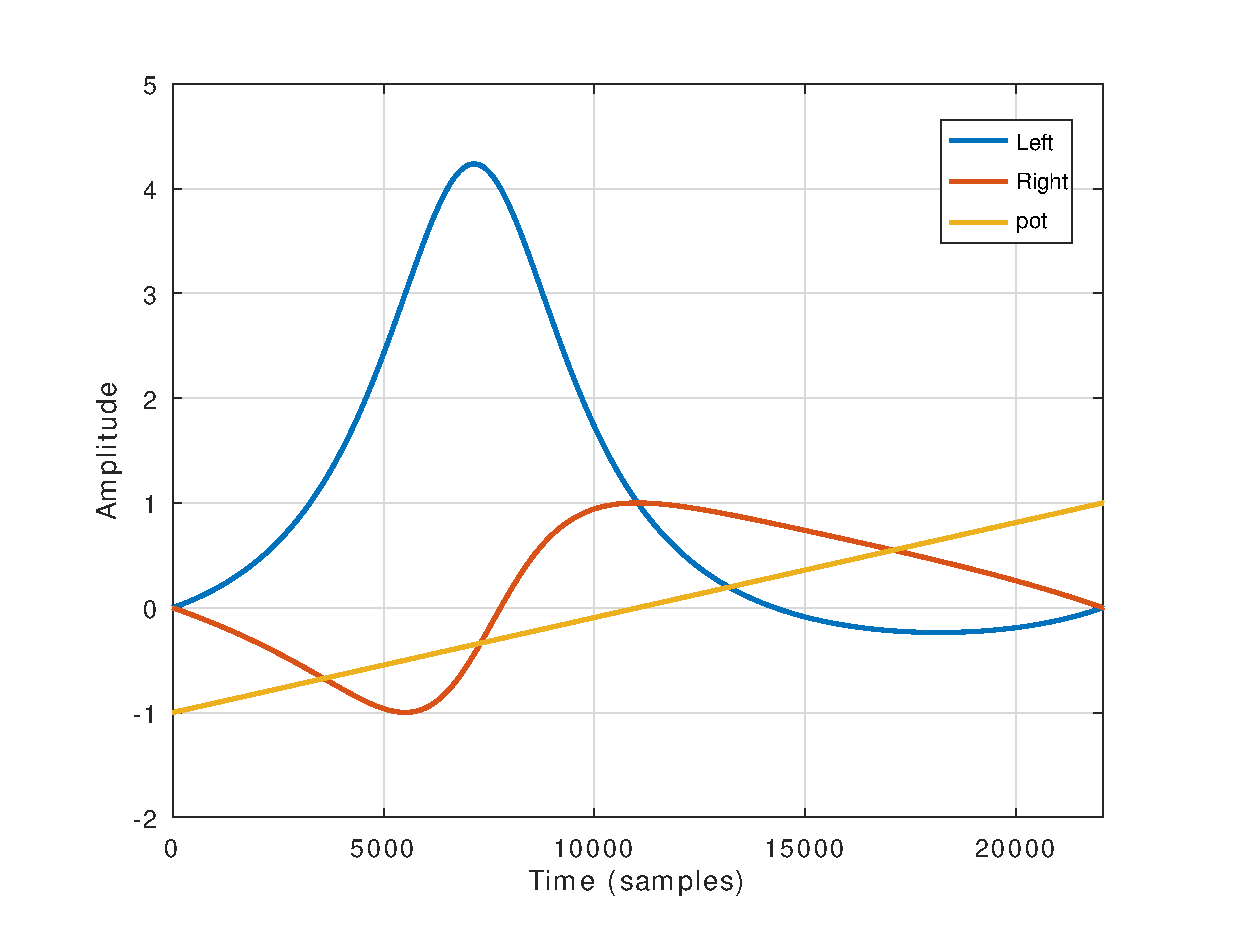
\includegraphics[width=1\columnwidth]{CAPITOLI/1000/IMG/mspanlrfbpot}
\caption{\textbf{Mid-Side to Left-Right panner}. The plot describes the feedback
response with a pan movement through the entire panorama, from -180 to 180
degrees (yellow line, normalized to -1 and 1). The energy multiplies up to four
times for the left channel in infinite feedback (blue line). The top of feedback
increasing is at 45 degrees position in direction of the channel in feedback.}
\label{fig:mspanlrfb}
\end{figure}
